\chapter{Neuroanatomical test}\label{chap:knowtest}

The following is the neurological knowledge test used in the research, prior to it a table with the solution and the participants answers.


% Please add the following required packages to your document preamble:
% \usepackage{graphicx}
% \usepackage[table,xcdraw]{xcolor}
% If you use beamer only pass "xcolor=table" option, i.e. \documentclass[xcolor=table]{beamer}
\begin{table}[H]
\centering
\resizebox{0.6\textwidth}{!}{%
\begin{tabular}{lll}
\rowcolor[HTML]{9698ED} 
\multicolumn{1}{c}{\cellcolor[HTML]{9698ED}Id} &
  \multicolumn{1}{c}{\cellcolor[HTML]{9698ED}Answers} &
  \multicolumn{1}{c}{\cellcolor[HTML]{9698ED}Score} \\
\rowcolor[HTML]{CBCEFB} 
\multicolumn{3}{c}{\cellcolor[HTML]{CBCEFB}First session} \\
1a &
  \begin{tabular}[c]{@{}l@{}}ccbcc cbadba cbbac badab babad\\ cbbac bbabca cabac baacc aabbb\end{tabular} &
  \begin{tabular}[c]{@{}l@{}}19\\ 17\end{tabular} \\
\rowcolor[HTML]{EFEFEF} 
1b &
  \begin{tabular}[c]{@{}l@{}}cbcba cbdddb cccac babad bdbad\\ cbcaa cbbddd cbcab babab bcbad\end{tabular} &
  \begin{tabular}[c]{@{}l@{}}15\\ 15\end{tabular} \\
1c &
  \begin{tabular}[c]{@{}l@{}}cbaaa cbaddd ccbac bdcad babab\\ ccaaa cbbbdd cbdac bdcad babab\end{tabular} &
  \begin{tabular}[c]{@{}l@{}}18\\ 16\end{tabular} \\
\rowcolor[HTML]{CBCEFB} 
\multicolumn{3}{c}{\cellcolor[HTML]{CBCEFB}Second session} \\
2a &
  \begin{tabular}[c]{@{}l@{}}ccdac bbbddd ccaac badad babca\\ ccaac bbbdda ccaac babad babcb\end{tabular} &
  \begin{tabular}[c]{@{}l@{}}13\\ 14\end{tabular} \\
\rowcolor[HTML]{EFEFEF} 
2b &
  \begin{tabular}[c]{@{}l@{}}cbdad dbbddd ccaac baadd bbddd\\ cbaac cbaddd ccbac baaab bbdad\end{tabular} &
  \begin{tabular}[c]{@{}l@{}}10\\ 17\end{tabular} \\
2c & \begin{tabular}[c]{@{}l@{}}ccdaa cbaddd ccbac baadd abbdd\\ ccbaa ccbaddd ccbac baabd bbbba\end{tabular} & \begin{tabular}[c]{@{}l@{}}12\\ 13\end{tabular} \\
\rowcolor[HTML]{EFEFEF} 
2d &
  \begin{tabular}[c]{@{}l@{}}cbdaa bdbddd ccaac bbdab cbcbb\\ ccaaa bbaddd ccacc bbadb babab\end{tabular} &
  \begin{tabular}[c]{@{}l@{}}10\\ 13\end{tabular} \\
2e &
  \begin{tabular}[c]{@{}l@{}}dddad acbddd cdaad daddd bccad\\ ccaac acaddd cccac baaad bbbcc\end{tabular} &
  \begin{tabular}[c]{@{}l@{}}6\\ 13\end{tabular} \\
\rowcolor[HTML]{CBCEFB} 
\multicolumn{3}{c}{\cellcolor[HTML]{CBCEFB}Solution} \\
 &
  cbcac cbabbb cabac bacab babab &
  26
\end{tabular}%
}
\end{table}

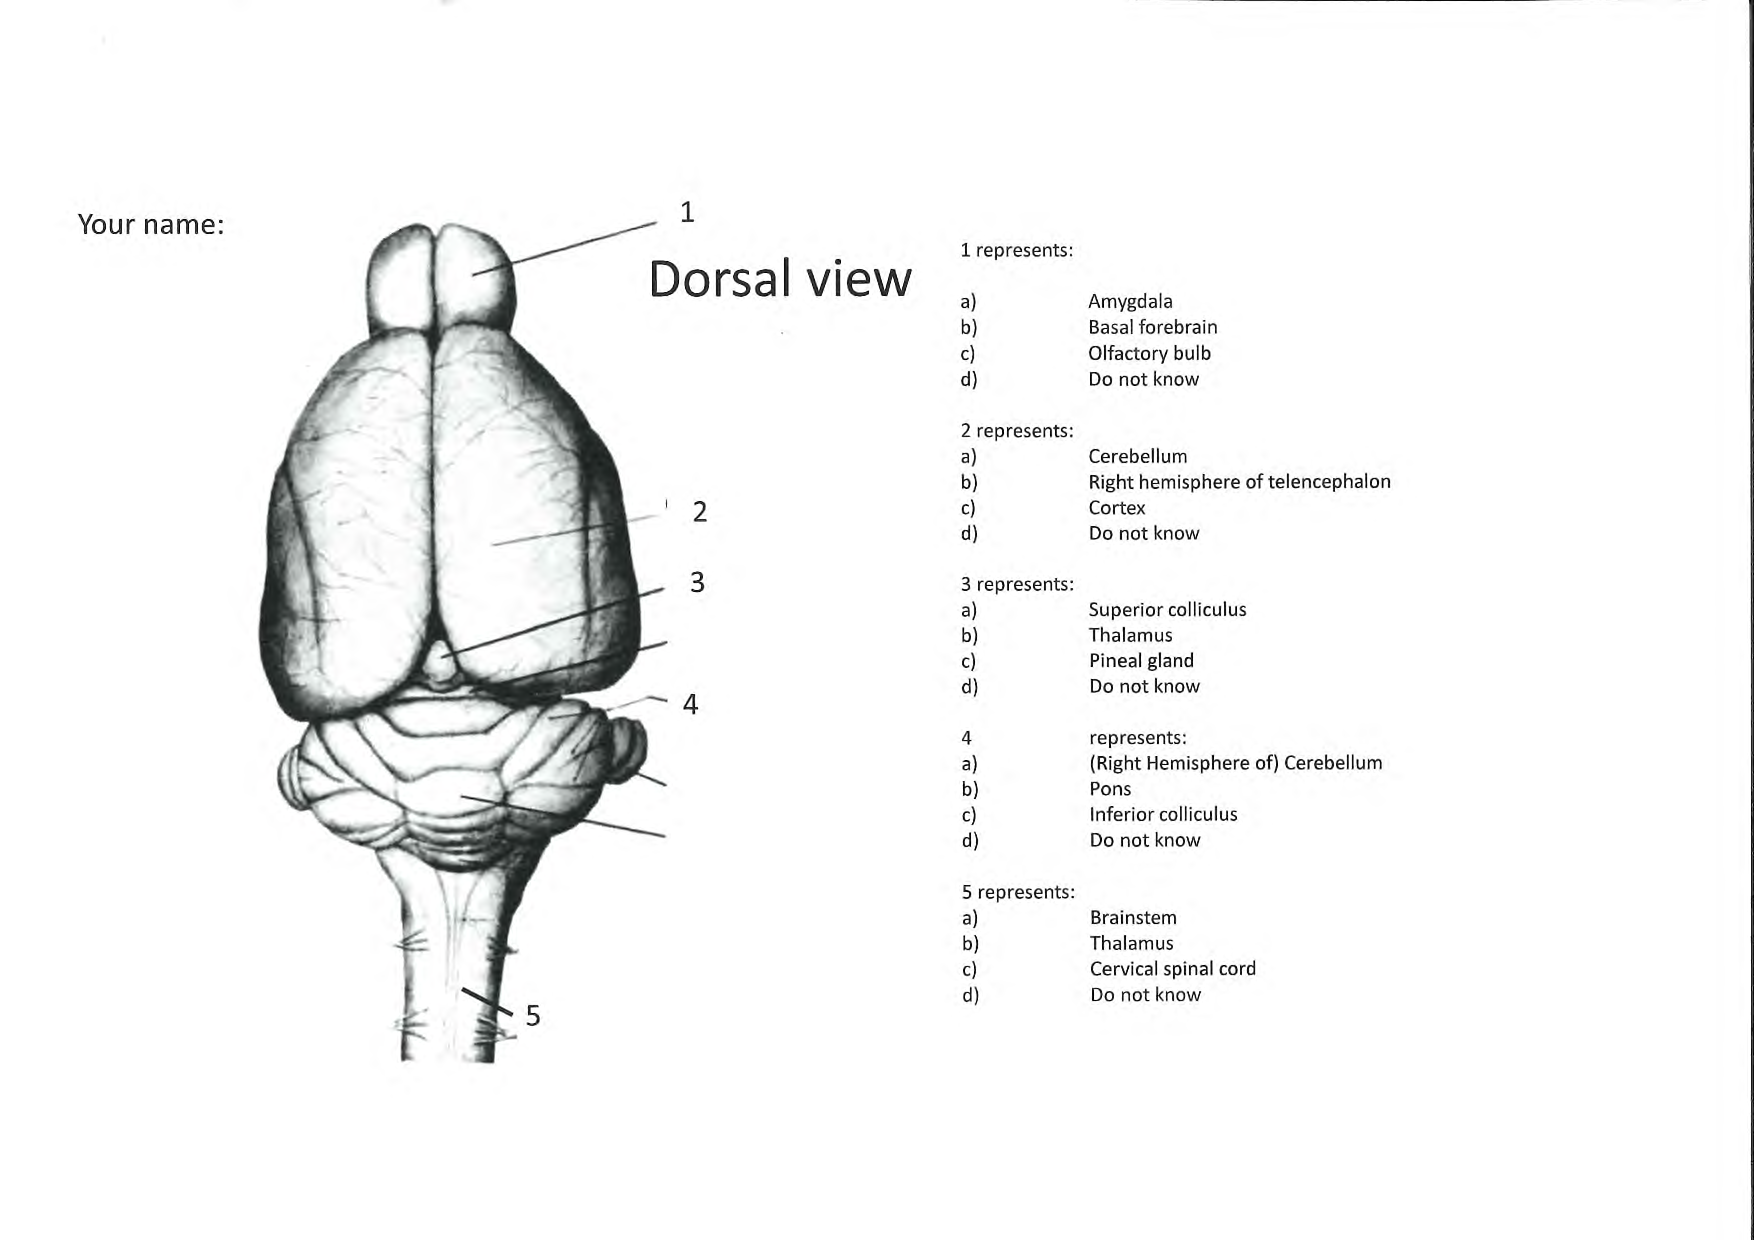
\includepdf[pages={1, 3-6}, angle=90]{appendix/knowtest}